% !TEX encoding = UTF-8 Unicode

\documentclass[a4paper, 12pt]{article}

\usepackage[T2A]{fontenc}
\usepackage[utf8x,utf8]{inputenc}
\usepackage[serbian]{babel}
\usepackage{amssymb}
\usepackage{amsmath}

\usepackage{color}
\usepackage{url}
\usepackage[unicode]{hyperref}
\hypersetup{colorlinks,citecolor=green,filecolor=green,linkcolor=blue,urlcolor=blue}
\usepackage{graphicx}
\graphicspath{ {./slike/} }

\begin{document}

%\title{\textbf{Slobodna bacanja}}
%\author{Matija Miličević, Jovana Rađenović}
%\subtitle{Seminarski rad iz predmeta Osnove matematičkog modeliranja}
%\date{maj 2019}
%\maketitle


\begin{titlepage}

\title{\textbf{Slobodna bacanja}}

\begin{center}
  \bfseries
  \large Matematički fakultet
  \vskip.2in
   Unvirezitet u Beogradu
  \vskip1.5in
  \emph{\huge Slobodna bacanja}
  \vskip.1in
  \small Seminarski rad iz predmeta \\Osnove matematičkog modeliranja
  \vskip.5in
  \large Matija Miličević \quad Jovana Rađenović
\end{center}

\vskip1.4in

\begin{minipage}{.3\textwidth}
  \begin{flushleft}
    \bfseries\large Profesor:\par \emph{Dr Milan Dražić}
  \end{flushleft}
\end{minipage}
\hskip.4\textwidth
\begin{minipage}{.3\textwidth}
  \begin{flushleft}
    \bfseries\large Asistent:\par \emph{Marija Ivanović}
  \end{flushleft}
\end{minipage}

\vskip1.7in

\centering
\bfseries
\Large maj 2019
\end{titlepage}

\pagebreak



\section{Zadatak}

Košarkaš prilikom slobodnog bacanja izbacuje loptu sa visine koja odgovara 5/4 sopstvene visine. Ako zanemarimo trenje vazduha, i ako je ugao bacanja $\theta$, da bi lopte prošle centrom obruča potrebna je brzina izbačaja $v_\theta$. Sa istom brzinom $v_\theta$ lopta će ući u koš i za bliske uglove $[\theta_1, \theta_2]$ (a da ne dodirne obruč). Za zadatu visinu košarkaša h odrediti onaj ugao bacanja $\theta$ koji obezbeđuje maksimalnu toleranciju $\theta_2 - \theta_1$. Rezultate tabelirati za omiljeni košarkaški klub ili reprezentaciju.

\subsection{Pojmovi}

Osnovni pojmovi:\\
$h$ - visina košarkaša koji izvodi slobodna bacanja;\\
$h_k$ - visina koša;\\
$\theta$ - ugao izbačaja;\\
$v_\theta$ - brzina izbačaja za ugao $\theta$ pri kojoj lopta prolazi kroz centar obruča;\\
$d_c$ - rastojanje od košarkaša (y-ose) do centra obruča;\\
$r_l$ - poluprečnik lopte;\\
$r_o$ - poluprečnik obruča ($r_o>r_l$);\\


\vskip1in
{\huge Ovde ce stajati slika sa pojmovima}
\vskip1in

%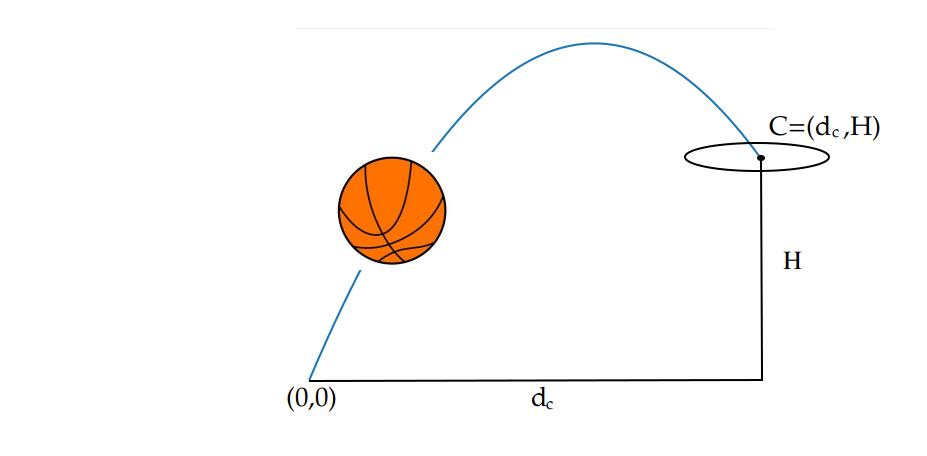
\includegraphics[width=7cm, height=4cm]{pic1} %TODO

\pagebreak



\section{Modeliranje leta lopte}

Podrazumevaćemo:
\begin{itemize}

%\item poluprečnik lopte $r_l$ je manji od poluprečnika obruča $r_o$:
%\[r_l<r_o\] %(3.1.1)

\item lopta ide dirketno ka košu, ne skreće sa putanje levo ili desno. Odnosno, nema lateralne greške pri šutu.

\item ugao $\theta$ je između $0^0$ i $90^0$:\\
\[0 < \theta < \pi/2\]

\item visina koša $h_k$ je veća od visine izbačaja košarkaša $\dfrac{_5}{^4}h$:\\
\[h_k > \dfrac{_5}{^4}h\]  %\hfill \centerline{}
%(ovo nije obavezno ali olakšava crtanje slike)\\

\end{itemize}


Posmatraćemo centar lopte kao materijalnu tačku $L = (x,y)$ koja počinje svoj put iz tačke $(x_0,y_0) = (0,\dfrac{_5}{^4}h)$. Da bi lopta prošla kroz centar obruča u jednom trenutku mora važiti $L = C$, gde je $C = (d_c,h_k)$.\\

Pošto su visina koša i košarkaša konstantne veličine možemo da transliramo ceo sistem tako da početna tačka centra lopte bude $L = (x_0,y_0) = (0,0)$, a tačka centra obruča $C = (d_c,h_k-\dfrac{_5}{^4}h)$.
Zbog jednostavnosti zapisa uzećemo da je $H = h_k-\dfrac{_5}{^4}h$, odnosno $C = (d_c,H)$.\\

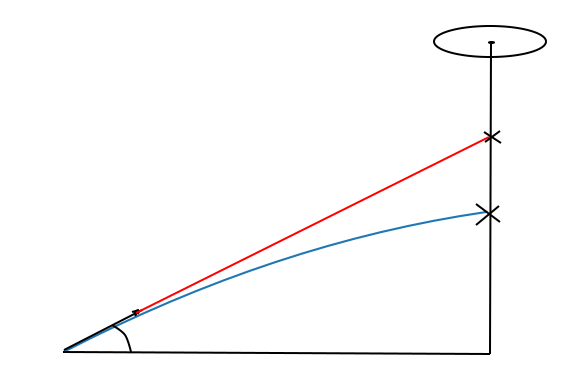
\includegraphics[width=10cm, height=5cm]{pic2}

Po ovoj slici možemo primetiti da je polazni problem u stvari jedna vrsta problema kosog hica.

\pagebreak



\subsection{Kretanje lopte}

Nakon što je bačena, možemo primetiti da na $x$-koordinatu lopte više ne utiče nijedna sila (otpor vazduha zanemarujemo), a pošto se lopta kreće brzinom zadatom pri šutu dolazimo do zaključka da važi:\\


\[x(t) = x_0 + v_{\theta x}\cdot t\]


Gde su: $x_0 = 0$; $v_{\theta x} = v_\theta \cdot \cos \theta$; odnosno:

\begin{equation}
x(t) = v_\theta \cdot \cos \theta \cdot t
\end{equation}

Sa druge strane na $y$-koordinatu sve vreme utiče gravitacija. Uz početnu brzinu zadatu šutom možemo da zaključimo da važi:

\[y(t) = y_0 + v_{\theta y} \cdot t - \dfrac{g \cdot t^2}{2}\]

gde je $g \approx 9.81\dfrac{_m}{^{s^2}}$. Pošto važi da su: $y_0 = 0$; $v_{\theta y} = v_\theta \cdot \sin \theta$; sledi:

\begin{equation}
y(t) = v_{\theta} \cdot \sin \theta\cdot t - \dfrac{g}{2} \cdot t^2
\end{equation}

Dakle, koordinate centra lopte $L$ u nekom trenutku $t$ su:

\[L(t) = (x(t), y(t)) = (v_\theta \cdot \cos \theta \cdot t, v_{\theta} \cdot \sin \theta \cdot t - \dfrac{g}{2} \cdot t^2)\]

\subsection{Odnos brzine, daljine i ugla} %TODO izbaciti cdot-ove?

Videli smo da položaj lopte zavisi od parametra vremena $t$. Nas zanima trenutak kada lopta prolazi kroz koš, odnosno $(x,y) = (d_c,H)$. Taj trenutak ćemo obeležiti sa $T$. Iz (1) i (2) sledi:

\[x(T) = v_\theta \cdot \cos \theta \cdot T = d_c\]

\[y(T) = v_{\theta} \cdot \sin \theta \cdot T - \dfrac{g}{2} \cdot T^2 = H\]

\pagebreak

Želimo da:

\begin{enumerate}
\item Nadjemo za ugao $\theta$ takvo $v_{\theta}$ da lopta prolazi kroz centar obruča $C$
\item Nadjemo najmanji ($\theta_1$) i najveći ($\theta_2$) ugao za koji lopta bačena tom brzinom $v_{\theta}$ i dalje upada u koš
\end{enumerate}

Da bismo našli $v_{\theta}$ koristimo prethodne dve jednačine. Iz prve jednačine:

\begin{equation}
T = \dfrac{d_c}{v_\theta \cos \theta}
\end{equation}

Dakle, vidimo odnos vremena i brzine. Gledamo sad drugu jednačinu:

\[v_{\theta} \sin \theta \cdot T - \dfrac{g}{2} \cdot T^2 = H\]

\[\dfrac{g}{2} \cdot T^2 - v_{\theta} \sin \theta \cdot T + H = 0\]

Iz ovoga dobijamo kvadratnu jednačinu po $T$:

\[T_{1,2} = \dfrac{v_{\theta} \sin \theta \pm \sqrt[]{v_{\theta}^2 \sin^2 \theta - 2 g H}}{g}\]

%Posmatramo putanju lopte kao kvadratnu funkciju po $T$.
%TODO dijagram preseka kv. funkcije i prave y = H

Možemo da vidimo da za vrednosti ${v_{\theta}^2 \sin^2 \theta < 2 g H}$ ne postoji rešenje u skupu realnih brojeva. To znači da lopta nikada neće dostići visinu H i samim tim nećemo postići koš.
U slučaju da važi ${v_{\theta}^2 \sin^2 \theta = 2 g H}$, postoji jedno rešenje $T_1 = T_2 = T$. Ovo nam isto ne odgovara jer ne prebacujemo visinu obruča. Samo ćemo uspeti da dobacimo do centra koša odozdo. Nećemo postići pogodak.

Na kraju dolazimo do konačnog slučaja ${v_{\theta}^2 \sin^2 \theta > 2 g H}$. Dobijamo dva rešenja $T_1$ i $T_2$. Ovo znači da je lopta u letu dosegla visinu H u trenutku $T_1$, dalje stigla do najviše tačke leta i pri padu u trenutku $T_2$ prošla savršeno kroz centar obruča. Pošto nas zanima trenutak prolaska kroz obruč uzimamo veće od dva $T$.

\begin{equation}
T = \dfrac{v_{\theta} \sin \theta + \sqrt[]{v_{\theta}^2 \sin^2 \theta - 2 g H}}{g}
\end{equation}

Takođe ćemo napomenuti da ubuduće važi uslov ${v_{\theta}^2 \sin^2 \theta > 2 g H}$, tj.

\begin{equation}
{\theta} > \arcsin(\sqrt[]{\dfrac{2 g H}{v_{\theta}^2}})
\end{equation}

\pagebreak

Nakon što izjednačimo $T$ iz (3) i (4) dobijamo:

\[\dfrac{d_c}{v_\theta \cos \theta} = \dfrac{v_{\theta} \sin \theta + \sqrt[]{v_{\theta}^2 \sin^2 \theta - 2 g H}}{g}\]

\[\dfrac{g d_c}{v_\theta \cos \theta} - v_{\theta} \sin \theta = \sqrt[]{v_{\theta}^2 \sin^2 \theta - 2 g H}\]

\[\dfrac{g^2 d_c^2}{v_\theta^2 \cos^2 \theta} - 2 g d_c \tan \theta + v_{\theta}^2 \sin^2 \theta = v_{\theta}^2 \sin^2 \theta - 2 g H\]


\[\dfrac{g^2 d_c^2}{v_\theta^2 \cos^2 \theta} - 2 g d_c \tan \theta + 2 g H = 0\]

Možemo ceo izraz da delimo sa $g$ jer znamo da je veće od 0:

\begin{equation}
\dfrac{g d_c^2}{v_\theta^2 \cos^2 \theta} - 2 d_c \tan \theta + 2 H = 0
\end{equation}

\[\dfrac{g d_c^2}{v_\theta^2 \cos^2 \theta} = 2 (d_c \tan \theta - H)\]

\[\dfrac{1}{v_\theta^2} = \dfrac{2 \cos^2 \theta (d_c \tan \theta - H)}{g d_c^2}\]

\[v_\theta^2 = \dfrac{g d_c^2}{2 \cos^2 \theta (d_c \tan \theta - H)}\]

\vskip.4in

Pošto znamo da važi $g$, $d$ > 0, sledi:

\begin{equation}
v_\theta = \sqrt[]{\dfrac{g d_c^2}{2 \cos^2 \theta (d_c \tan \theta - H)}}
\end{equation}

\vskip.2in

Ovo inače predstavlja brzinu neophodnu da bi lopta pri padu prošla kroz tačku $(d_c,H)$. Naravno pri uslovu da se šutira pod uglom $\theta$.
Tokom sređivanja izraza došli smo do novog uslova $d_c \tan \theta - H > 0$, odnosno:

\begin{equation}
{\theta} > \arctan(\dfrac{H}{d_c})
\end{equation}

\pagebreak

Što je geometrijski logično jer da ne važi ovaj uslov mi bi ciljali ispod koša i uvek bi prebacili daljinu obruča pre nego što bi stigli na njegovu visinu.

%TODO slika!
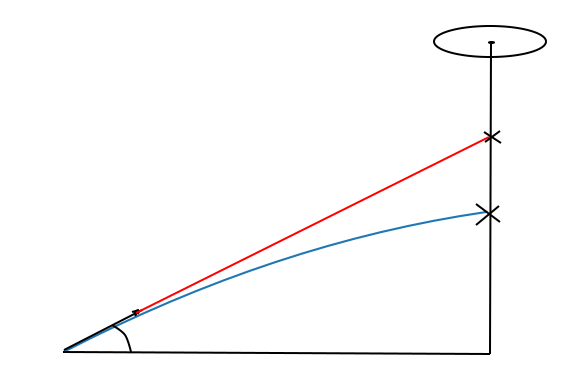
\includegraphics[width=10cm, height=5cm]{pic3}


Izjednačavanjem (3) i (4) možemo da izvedemo još dve formule. Do prve dolazimo putem:

\[\dfrac{d_c}{v_\theta \cos \theta} = \dfrac{v_{\theta} \sin \theta + \sqrt[]{v_{\theta}^2 \sin^2 \theta - 2 g H}}{g}\]

\[d_c = v_\theta \cos \theta (\dfrac{v_{\theta} \sin \theta + \sqrt[]{v_{\theta}^2 \sin^2 \theta - 2 g H}}{g})\]

Odnosno:

\begin{equation}
d = \dfrac{v \cos \theta}{g}(v \sin \theta + \sqrt[]{v^2 \sin^2 \theta - 2 g H})
\end{equation}

\vskip.2in

Gde smo namerno zamenili $d_c$ i $v_\theta$ sa $d$ i $v$, jer formula važi za proizvoljne pozitivne vrednosti. Ovom formulom možemo da izračunamo daljinu koju će lopta preći pri šutu sa početnom brzinom $v$ i uglom $\theta$, pre nego što padne na visinu $H$. Jasno je da formulu (7) takođe možemo da tumačimo sa proizvoljnim $d$ umesto daljine do sredine koša. Videćemo kasnije svrhu ovih formula.

Drugu formulu dobijamo iz (6):

\[ \dfrac{g d^2}{v^2 \cos^2 \theta} - 2 d \tan \theta + 2 H = 0 \]

\[ \dfrac{g d^2 (1 + \tan^2 \theta)}{v^2} - 2 d \tan \theta + 2 H = 0 \]

\[ \dfrac{g d^2}{v^2} \tan^2 \theta - 2 d \tan \theta + 2 H + \dfrac{g d^2}{v^2} = 0 \]

\pagebreak

\[ g d^2 \tan^2 \theta - 2 d v^2 \tan \theta + 2 H + g d^2 = 0 \]

Ovo je očigledno kvadratna jednačina po $\tan \theta$:

\[ \tan \theta = \dfrac{2 d v^2 \pm \sqrt[]{4 d^2 v^4 - 4 (g d^2)(2 H + g d^2)}}{2 g d^2} \]

Nakon izvlačenja $2d$ ispred korena i skraćivanja:

\[ \tan \theta = \dfrac{v^2 \pm \sqrt[]{v^4 - g(2 H - g d^2)}}{g d} \]

\begin{equation}
\theta = \arctan (\dfrac{v^2 \pm \sqrt[]{v^4 - g(2 H - g d^2)}}{g d})
\end{equation}

Ovom formulom možemo da odredimo pod kojim uglom je potrebno izbaciti loptu da bi pri brzini $v$ prešla put $d$ pre nego što se spusti na visinu $H$.
Očigledno ako važi $v^4 - g(2 H - g d^2) < 0$ brzina lopte je premala da bi prešla daljinu $d$ pre nego što padne ispod $H$. U slučaju $v^4 - g(2 H - g d^2) = 0$ postoji jedan ugao $\theta$ kojim postižemo ovu daljinu, a za $v^4 - g(2 H - g d^2) > 0$ postoje dva ugla.


%TODO SLIKA!!!!! + legenda

\vskip1in
{\huge Ovde ce stajati dijagram dva ugla}
\vskip1in


Sa formulama (7), (9) i (10) možemo da vidimo odnos brzine, daljine i ugla pri putanji naše lopte.

\pagebreak



\section{Uslovi za prolazak lopte kroz obruč} %TODO

Do sada smo loptu posmatrali kao tačku u 2-D prostoru $L = (x,y)$. Odredili smo dva uslova koja moraju biti ispunjena da bi lopta prošla kroz obruč:

\[{\theta} > \arcsin(\sqrt[]{\dfrac{2 g H}{v_{\theta}^2}}) \quad (5), \quad {\theta} > \arctan(\dfrac{H}{d_c}) \quad (8) \]

Pre nego što se pozabavimo traženjem uglova $\theta_1$ i $\theta_2$ moramo da vidimo koji još uslovi moraju biti ispunjeni da bi lopta upala u koš. Po postavci zadatka nas samo zanimaju slučajevi kada lopta ne dodiruje obruč, odbici koji ulaze u koš se ne priznaju. Pošto podrazumevamo da nema lateralne greške nas samo zanima prednji i zadnji deo obruča.

Da bi lopta prošla kroz obruč u trenutku $T$ ($y = H$) udaljenost njenog centra od prednjeg i zadnjeg dela obruča mora biti veća od poluprečnika lopte $r_l$, ali njen centar mora i dalje biti izmedju ove dve tačke. Koordinatne tačke ovih delova obruča možemo lako odrediti. Ako je centar obruča $C = (d_c,H)$, a poluprečnik obruča $r_o$, onda je bliži deo obruča $O_1 = (d_c - r_o, H)$, a dalji deo obruča $O_2 = (d_c + r_o, H)$.

Pošto je na svom putu lopta krenula da pada, možemo da primetimo da kako se njena $x$-koordinata povećava, tako se $y$-koordinata smanjuje. To znači da u trenutku $T$ ona će imati maksimalnu $x$-koordinatu pre nego što prođe (ili ne prođe) kroz obruč, tj. $L = (x_{max},H)$. Dakle da bi lopta u trenutku $T$ prošla kroz obruč mora da važi:

\[ d_c - r_o < x_{max} - r_l \quad \land \quad x_{max} + r_l < d_c + r_o \]

%Odnosno:

\[d_c - r_o + r_l \quad < \quad x_{max} \quad < \quad d_c - r_l + r_o \]

%\vskip.2in

Ubuduće ćemo ove dve tačke zapisivati kao $d_1 = d_c - r_o + r_l$ i $d_2 = d_c - r_l + r_o$

\begin{equation}
d_1 < x_{max} < d_2
\end{equation}

Ovo je bio uslov prolaska lopte u trenutku $T$. Nas sad zanima da li je lopta mogla udariti u obruč pre tog trenutka. Za dalji deo obruča očigledno je odgovor ne, jer ako centar lopte nije prebacio tačku $d_2$ u trenutku $T$ sigurno nije ni u nekom ranijem trenutku kada je lopta bila udaljenija od $O_2$. Dalje se logično postavlja pitanje za $O_1$.


\[TODO!!!\]


\pagebreak



\section{Uglovi $\theta_1$ i $\theta_2$} %TODO

Pretpostavimo da $\theta \subseteq (0,\pi/2)$ ispunjava uslove i može se pogoditi koš ako šutiramo pod tim uglom. Postavlja se pitanje kako da odredimo $\theta_1$ i $\theta_2$ za dati ugao $\theta$?

Očigledan način je da iskoristimo formulu (10).

Druga opcija je iterativni metod.

\[TODO!!!\]



\section{Model rešenja: Iterativni metod} %TODO

Jednostavan i očigledan model rešenja je da za svaki mogući ugao $\theta$ nadjemo $\theta_1$ i $\theta_2$ i da kao optimalni ugao izaberemo onaj čija je razlika
$\theta_2 - \theta_1$ maksimalna.

\vskip.2in

\[TODO!!!\]

Vremenska složenost ovog rešenja je na taj način $O(n \cdot m)$ gde je $n$ broj uglova $\theta$, a $m$ prosek broja uglova $\theta_1$ i $\theta_2$. Naravno pošto uglovi pripadaju neprebrojivom skupu nećemo moći da proverimo rešenje za svaki ugao $\theta$. Moraćemo da diskretizujemo problem time što ćemo odrediti korak iteracije. Manji korak znači veća preciznost, ali i duži rad programa.

\[TODO!!! + KOD!\]

\end{document}